\documentclass[tikz]{standalone}
\usetikzlibrary{arrows,calc,shapes,decorations.pathreplacing}
\begin{document}
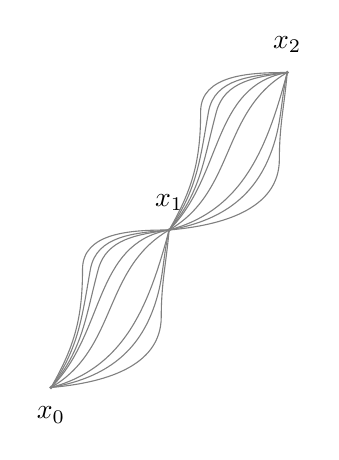
\begin{tikzpicture}[scale=.5]
\fill[gray] (6,0) circle (1.3pt);
  \node[label=below:$x_0$]  (x1) at (6,0)  {}; % {$\bullet$};
  \fill[gray] (9,4) circle (1.3pt);
  \node[label=above:$x_1$]  (x0) at (9,4)  {}; % {$\bullet$};  
%  \node[label=above:$x_1$]  (x0) at (9,4)  {$\bullet$};  
  \draw[gray] (x1.center) to [out=5,in=-90]++(2.8,1.8) to[out=90,in=-95](x0.center);
  \draw[gray] (x1.center) to [out=10,in=-110]++(2.6,2) to[out=70,in=-103](x0.center); 
  \draw[gray] (x1.center) to [out=15,in=-105](x0.center);
  \draw[gray] (x1.center) to [out=30,in=-150](x0.center);
  \draw[gray] (x1.center) to [out=45,in=-170](x0.center); 
  \draw[gray] (x1.center) to [out=50,in=-105]++(1.2,3)to [out=75,in=-172](x0.center); 
  \draw[gray] (x1.center) to [out=55,in=-100]++(1.0,3) to[out=80,in=-175](x0.center); 
  \draw[gray] (x1.center) to [out=60,in=-90]++(0.8,3) to[out=90,in=-180] (x0.center);
\begin{scope}[shift={(3,4)}]
\fill[gray] (6,0) circle (1.3pt);
  \node%[label=below:$x_1$]  
  	(x1) at (6,0) {};%  {$\bullet$};
%  \node[label=above:$x_2$]  (x0) at (9,4)  {$\bullet$};  
\fill[gray] (9,4) circle (1.3pt);
  \node[label=above:$x_2$]  (x0) at (9,4)  {}; % {$\bullet$};  
  \draw[gray] (x1.center) to [out=5,in=-90]++(2.8,1.8) to[out=90,in=-95](x0.center);
  \draw[gray] (x1.center) to [out=10,in=-110]++(2.6,2) to[out=70,in=-103](x0.center); 
  \draw[gray] (x1.center) to [out=15,in=-105](x0.center);
  \draw[gray] (x1.center) to [out=30,in=-150](x0.center);
  \draw[gray] (x1.center) to [out=45,in=-170](x0.center); 
  \draw[gray] (x1.center) to [out=50,in=-105]++(1.2,3)to [out=75,in=-172](x0.center); 
  \draw[gray] (x1.center) to [out=55,in=-100]++(1.0,3) to[out=80,in=-175](x0.center); 
  \draw[gray] (x1.center) to [out=60,in=-90]++(0.8,3) to[out=90,in=-180] (x0.center);
\end{scope}
\end{tikzpicture}
\end{document}
